\documentclass[twoside]{book}

% Packages required by doxygen
\usepackage{fixltx2e}
\usepackage{calc}
\usepackage{doxygen}
\usepackage[export]{adjustbox} % also loads graphicx
\usepackage{graphicx}
\usepackage[utf8]{inputenc}
\usepackage{makeidx}
\usepackage{multicol}
\usepackage{multirow}
\PassOptionsToPackage{warn}{textcomp}
\usepackage{textcomp}
\usepackage[nointegrals]{wasysym}
\usepackage[table]{xcolor}

% Font selection
\usepackage[T1]{fontenc}
\usepackage[scaled=.90]{helvet}
\usepackage{courier}
\usepackage{amssymb}
\usepackage{sectsty}
\renewcommand{\familydefault}{\sfdefault}
\allsectionsfont{%
  \fontseries{bc}\selectfont%
  \color{darkgray}%
}
\renewcommand{\DoxyLabelFont}{%
  \fontseries{bc}\selectfont%
  \color{darkgray}%
}
\newcommand{\+}{\discretionary{\mbox{\scriptsize$\hookleftarrow$}}{}{}}

% Page & text layout
\usepackage{geometry}
\geometry{%
  a4paper,%
  top=2.5cm,%
  bottom=2.5cm,%
  left=2.5cm,%
  right=2.5cm%
}
\tolerance=750
\hfuzz=15pt
\hbadness=750
\setlength{\emergencystretch}{15pt}
\setlength{\parindent}{0cm}
\setlength{\parskip}{3ex plus 2ex minus 2ex}
\makeatletter
\renewcommand{\paragraph}{%
  \@startsection{paragraph}{4}{0ex}{-1.0ex}{1.0ex}{%
    \normalfont\normalsize\bfseries\SS@parafont%
  }%
}
\renewcommand{\subparagraph}{%
  \@startsection{subparagraph}{5}{0ex}{-1.0ex}{1.0ex}{%
    \normalfont\normalsize\bfseries\SS@subparafont%
  }%
}
\makeatother

% Headers & footers
\usepackage{fancyhdr}
\pagestyle{fancyplain}
\fancyhead[LE]{\fancyplain{}{\bfseries\thepage}}
\fancyhead[CE]{\fancyplain{}{}}
\fancyhead[RE]{\fancyplain{}{\bfseries\leftmark}}
\fancyhead[LO]{\fancyplain{}{\bfseries\rightmark}}
\fancyhead[CO]{\fancyplain{}{}}
\fancyhead[RO]{\fancyplain{}{\bfseries\thepage}}
\fancyfoot[LE]{\fancyplain{}{}}
\fancyfoot[CE]{\fancyplain{}{}}
\fancyfoot[RE]{\fancyplain{}{\bfseries\scriptsize Generated by Doxygen }}
\fancyfoot[LO]{\fancyplain{}{\bfseries\scriptsize Generated by Doxygen }}
\fancyfoot[CO]{\fancyplain{}{}}
\fancyfoot[RO]{\fancyplain{}{}}
\renewcommand{\footrulewidth}{0.4pt}
\renewcommand{\chaptermark}[1]{%
  \markboth{#1}{}%
}
\renewcommand{\sectionmark}[1]{%
  \markright{\thesection\ #1}%
}

% Indices & bibliography
\usepackage{natbib}
\usepackage[titles]{tocloft}
\setcounter{tocdepth}{3}
\setcounter{secnumdepth}{5}
\makeindex

% Hyperlinks (required, but should be loaded last)
\usepackage{ifpdf}
\ifpdf
  \usepackage[pdftex,pagebackref=true]{hyperref}
\else
  \usepackage[ps2pdf,pagebackref=true]{hyperref}
\fi
\hypersetup{%
  colorlinks=true,%
  linkcolor=blue,%
  citecolor=blue,%
  unicode%
}

% Custom commands
\newcommand{\clearemptydoublepage}{%
  \newpage{\pagestyle{empty}\cleardoublepage}%
}

\usepackage{caption}
\captionsetup{labelsep=space,justification=centering,font={bf},singlelinecheck=off,skip=4pt,position=top}

%===== C O N T E N T S =====

\begin{document}

% Titlepage & ToC
\hypersetup{pageanchor=false,
             bookmarksnumbered=true,
             pdfencoding=unicode
            }
\pagenumbering{roman}
\begin{titlepage}
\vspace*{7cm}
\begin{center}%
{\Large Practica }\\
\vspace*{1cm}
{\large Generated by Doxygen 1.8.11}\\
\end{center}
\end{titlepage}
\clearemptydoublepage
\tableofcontents
\clearemptydoublepage
\pagenumbering{arabic}
\hypersetup{pageanchor=true}

%--- Begin generated contents ---
\chapter{Save\+Pass Daniel\+Segura (aplicacio)}
\label{index}\hypertarget{index}{}\hypertarget{index_intro_sec}{}\section{Introduction}\label{index_intro_sec}
This program was developed to store your passwords, during m08 uf 4 \hypertarget{index_compile_sec}{}\section{Compilation}\label{index_compile_sec}
To compile this program, use gcc \hyperlink{aplicacio_8c}{aplicacio.\+c} -\/o aplicacio 
\chapter{File Index}
\section{File List}
Here is a list of all documented files with brief descriptions\+:\begin{DoxyCompactList}
\item\contentsline{section}{\hyperlink{aplicacio_8c}{aplicacio.\+c} }{\pageref{aplicacio_8c}}{}
\end{DoxyCompactList}

\chapter{File Documentation}
\hypertarget{aplicacio_8c}{}\section{aplicacio.\+c File Reference}
\label{aplicacio_8c}\index{aplicacio.\+c@{aplicacio.\+c}}
{\ttfamily \#include $<$stdio.\+h$>$}\\*
{\ttfamily \#include $<$stdlib.\+h$>$}\\*
{\ttfamily \#include $<$string.\+h$>$}\\*
Include dependency graph for aplicacio.\+c\+:\nopagebreak
\begin{figure}[H]
\begin{center}
\leavevmode
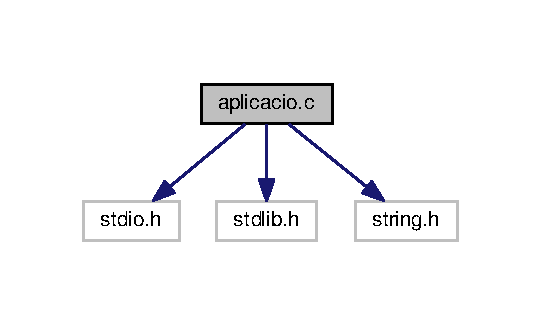
\includegraphics[width=260pt]{aplicacio_8c__incl}
\end{center}
\end{figure}
\subsection*{Functions}
\begin{DoxyCompactItemize}
\item 
void \hyperlink{aplicacio_8c_a3cbbab60b4ba9c8407fc6ab9a9ddec9e}{get\+\_\+password} ()
\begin{DoxyCompactList}\small\item\em This function is the option c) of the menu\+: get\+\_\+password. \end{DoxyCompactList}\item 
void \hyperlink{aplicacio_8c_a404566d1a8e7b270869258e3c71acfa3}{list\+\_\+usernames} ()
\begin{DoxyCompactList}\small\item\em This function is the option b) of the menu\+: list\+\_\+usernames. \end{DoxyCompactList}\item 
void \hyperlink{aplicacio_8c_a62104a76feeb098aa005353fc584a1d6}{add\+\_\+password} ()
\begin{DoxyCompactList}\small\item\em This function is the option a) of the menu\+: add\+\_\+password. \end{DoxyCompactList}\item 
int \hyperlink{aplicacio_8c_ae66f6b31b5ad750f1fe042a706a4e3d4}{main} ()
\begin{DoxyCompactList}\small\item\em Main function. \end{DoxyCompactList}\end{DoxyCompactItemize}


\subsection{Detailed Description}
\begin{DoxyAuthor}{Author}
Daniel Segura 
\end{DoxyAuthor}
\begin{DoxyVersion}{Version}
1.\+0 
\end{DoxyVersion}
\begin{DoxyDate}{Date}
2019-\/06-\/04 
\end{DoxyDate}
\begin{DoxyWarning}{Warning}
aixo es el arxiu del guillem perque no recordo res de c 
\end{DoxyWarning}
\begin{DoxyCopyright}{Copyright}
G\+NU Public License 
\end{DoxyCopyright}


\subsection{Function Documentation}
\index{aplicacio.\+c@{aplicacio.\+c}!add\+\_\+password@{add\+\_\+password}}
\index{add\+\_\+password@{add\+\_\+password}!aplicacio.\+c@{aplicacio.\+c}}
\subsubsection[{\texorpdfstring{add\+\_\+password()}{add_password()}}]{\setlength{\rightskip}{0pt plus 5cm}void add\+\_\+password (
\begin{DoxyParamCaption}
{}
\end{DoxyParamCaption}
)}\hypertarget{aplicacio_8c_a62104a76feeb098aa005353fc584a1d6}{}\label{aplicacio_8c_a62104a76feeb098aa005353fc584a1d6}


This function is the option a) of the menu\+: add\+\_\+password. 

Asks the user to input a description, username and password, then opens the file and stores the data \begin{DoxyReturn}{Returns}
doesn\textquotesingle{}t return anything, its a void 
\end{DoxyReturn}
Pointer to the file that stores passwords \index{aplicacio.\+c@{aplicacio.\+c}!get\+\_\+password@{get\+\_\+password}}
\index{get\+\_\+password@{get\+\_\+password}!aplicacio.\+c@{aplicacio.\+c}}
\subsubsection[{\texorpdfstring{get\+\_\+password()}{get_password()}}]{\setlength{\rightskip}{0pt plus 5cm}void get\+\_\+password (
\begin{DoxyParamCaption}
{}
\end{DoxyParamCaption}
)}\hypertarget{aplicacio_8c_a3cbbab60b4ba9c8407fc6ab9a9ddec9e}{}\label{aplicacio_8c_a3cbbab60b4ba9c8407fc6ab9a9ddec9e}


This function is the option c) of the menu\+: get\+\_\+password. 

Prints in screen the password of the username the user inputted 
\begin{DoxyParams}{Parameters}
{\em test\+\_\+param} & this param doesnt exist, its just a test for dogygen \\
\hline
\end{DoxyParams}
\begin{DoxyReturn}{Returns}
doesn\textquotesingle{}t return anything, its a void 
\end{DoxyReturn}
Pointer to the file that stores passwords

This string stores every line of the file.\+txt

Variable found is used for some stuff

We store the username of the password we want here \index{aplicacio.\+c@{aplicacio.\+c}!list\+\_\+usernames@{list\+\_\+usernames}}
\index{list\+\_\+usernames@{list\+\_\+usernames}!aplicacio.\+c@{aplicacio.\+c}}
\subsubsection[{\texorpdfstring{list\+\_\+usernames()}{list_usernames()}}]{\setlength{\rightskip}{0pt plus 5cm}void list\+\_\+usernames (
\begin{DoxyParamCaption}
{}
\end{DoxyParamCaption}
)}\hypertarget{aplicacio_8c_a404566d1a8e7b270869258e3c71acfa3}{}\label{aplicacio_8c_a404566d1a8e7b270869258e3c71acfa3}


This function is the option b) of the menu\+: list\+\_\+usernames. 

Prints in screen all the combinations of description + usernames \begin{DoxyReturn}{Returns}
doesn\textquotesingle{}t return anything, its a void 
\end{DoxyReturn}
Pointer to the file that stores passwords

This string stores every line of the file.\+txt \index{aplicacio.\+c@{aplicacio.\+c}!main@{main}}
\index{main@{main}!aplicacio.\+c@{aplicacio.\+c}}
\subsubsection[{\texorpdfstring{main()}{main()}}]{\setlength{\rightskip}{0pt plus 5cm}int main (
\begin{DoxyParamCaption}
{}
\end{DoxyParamCaption}
)}\hypertarget{aplicacio_8c_ae66f6b31b5ad750f1fe042a706a4e3d4}{}\label{aplicacio_8c_ae66f6b31b5ad750f1fe042a706a4e3d4}


Main function. 

This function prints a menu, and depending on the choice of the user, does one function and then exits the program \begin{DoxyReturn}{Returns}
returns 0 if successfull 
\end{DoxyReturn}

%--- End generated contents ---

% Index
\backmatter
\newpage
\phantomsection
\clearemptydoublepage
\addcontentsline{toc}{chapter}{Index}
\printindex

\end{document}
